\documentclass[calcdimensions,landscape,letterpaper]{powersem}
\usepackage{color}
\usepackage[pdftex]{thumbpdf} % For thumbnails
\usepackage[pdftex]{hyperref} % For links.
\usepackage[display,coloremph,whitebackground]{texpower} % colormath
\usepackage{fixseminar}
\usepackage{tpslifonts}
\usepackage[pdftex,final]{graphicx} % For including graphics.
\usepackage[utf8]{inputenc}
\usepackage{minted}
\usepackage{amsmath}
\usepackage{amssymb}
\usepackage{eurosym}
\usepackage{booktabs} % rules in tables
\usepackage{multirow} % multi-row cells
\usepackage{rotating} % text rotation

\title{A Short Introduction to OpenGL}
\author{Jan Wedekind}
\date{Thursday, May 30th 2024}

\DeclareGraphicsExtensions{.jpg,.pdf,.png}
\pdfcompresslevel=9

\hypersetup{
   pdftitle          = {\thetitle},
   pdfsubject        = {After Catchup Presentation 30th May 2024},
   pdfauthor         = {Jan Wedekind},
   pdfkeywords       = {opengl, graphics, software},
   pdfcreator        = {okular},
   pdfproducer       = {LaTeX with hyperref and thumbpdf},
   bookmarksopen     = false,
   bookmarksnumbered = true,
   colorlinks        = true,
   pdfstartpage      = {1},
   pdfpagemode       = {FullScreen}
}

\DeclarePanel{top}{
  \begin{picture}(0,0)
    \put(-3, -293){\resizebox*{\pdfpagewidth}{\pdfpageheight}{
\includegraphics{slide.png}}}
    \put(-10,-20){\parbox[c]{.9\textwidth}{\center\large\bf\thecurrentheading}}
  \end{picture}
}

\DeclarePanel{bottom}{
  \begin{picture}(0,0)
    \put(0,15){\parbox[c]{.98\pdfpagewidth}{\tiny\thedate\hfill\theslide/22}}
  \end{picture}
}

\slidesmag{4}
\backgroundstyle{none}
\slideframe{none}
\pagestyle{empty}

\mklength{\slideleftmargin}{-2cm}
\mklength{\sliderightmargin}{-2cm}
\mklength{\slidetopmargin}{2.0cm}
\mklength{\slidebottommargin}{1.5cm}

\renewcommand{\currentpagevalue}{\value{slide}}
\newcommand{\thecurrentheading}{}
\newcommand{\heading}[1]{\renewcommand{\thecurrentheading}{#1}}
\newcommand{\subheading}[1]{\concept{#1}}

\begin{document}

\begin{slide}
  \pdfbookmark[1]{\thetitle}{title}
  \heading{\ }
  \begin{center}
    \maketitle
  \end{center}
\end{slide}

\begin{slide}
  \pdfbookmark[1]{Motivation}{motivation}
  \heading{Motivation}
  \begin{center}
    \resizebox*{.5\textwidth}{!}{
\includegraphics{logo}}\bigskip\\
    \begin{minipage}[c]{.95\textwidth}
      \begin{itemize}
          \item OpenGL is cross-platform
          \item OpenGL is less verbose than Vulkan, but OpenGL knowledge transfers to Vulkan
          \item Use GLFW\footnote{\url{https://www.glfw.org/}} for cross-platform windows and events
          \item GLFW and OpenGL have bindings for many languages
          \item See QGLWidget\footnote{\url{https://doc.qt.io/qt-5/qglwidget.html}} for using OpenGL with Qt
      \end{itemize}
    \end{minipage}
  \end{center}
\end{slide}

\begin{slide}
  \pdfbookmark[1]{Showcase}{showcase}
  \heading{Showcase}
  \begin{center}
    \begin{minipage}[c]{.47\textwidth}
      \begin{center}
        \resizebox*{\textwidth}{!}{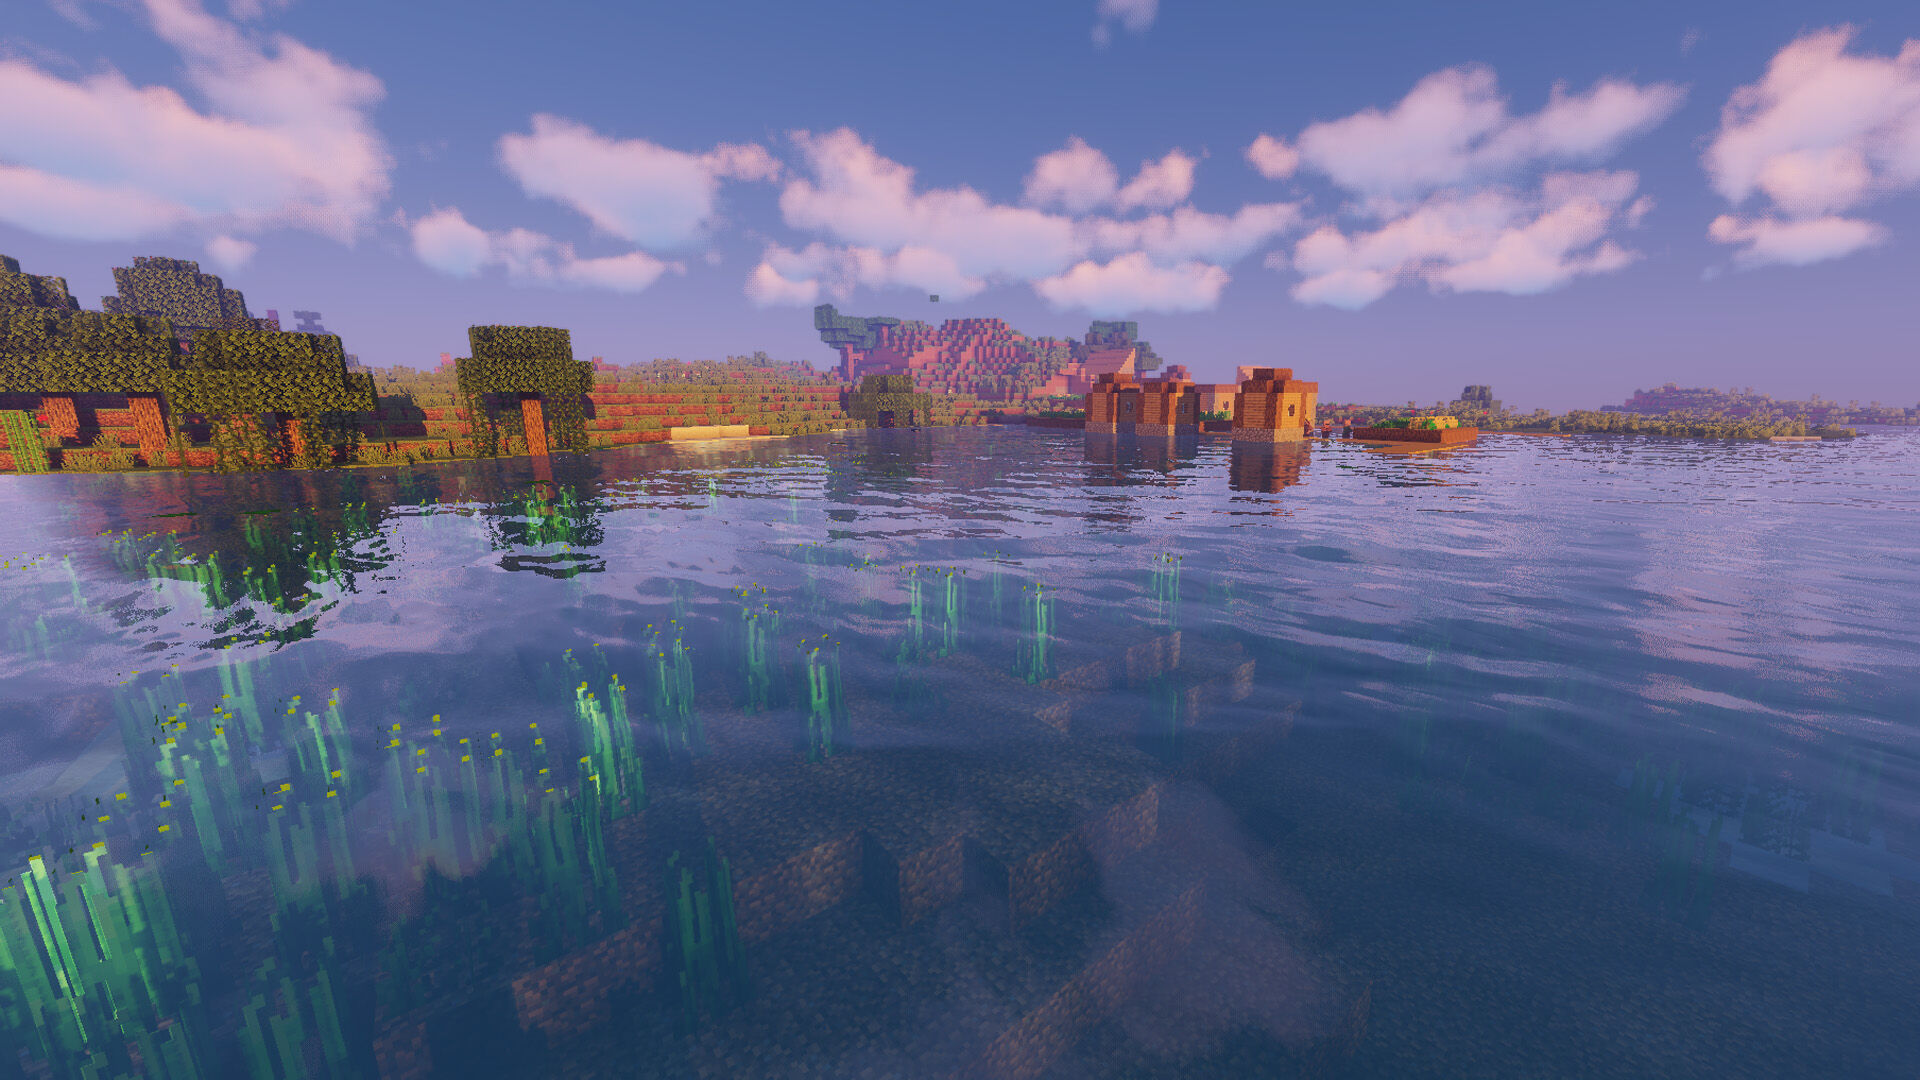
\includegraphics{minecraft}}\\
        Minecraft Java Edition
      \end{center}
    \end{minipage}
    \begin{minipage}[c]{.47\textwidth}
      \begin{center}
        \resizebox*{\textwidth}{!}{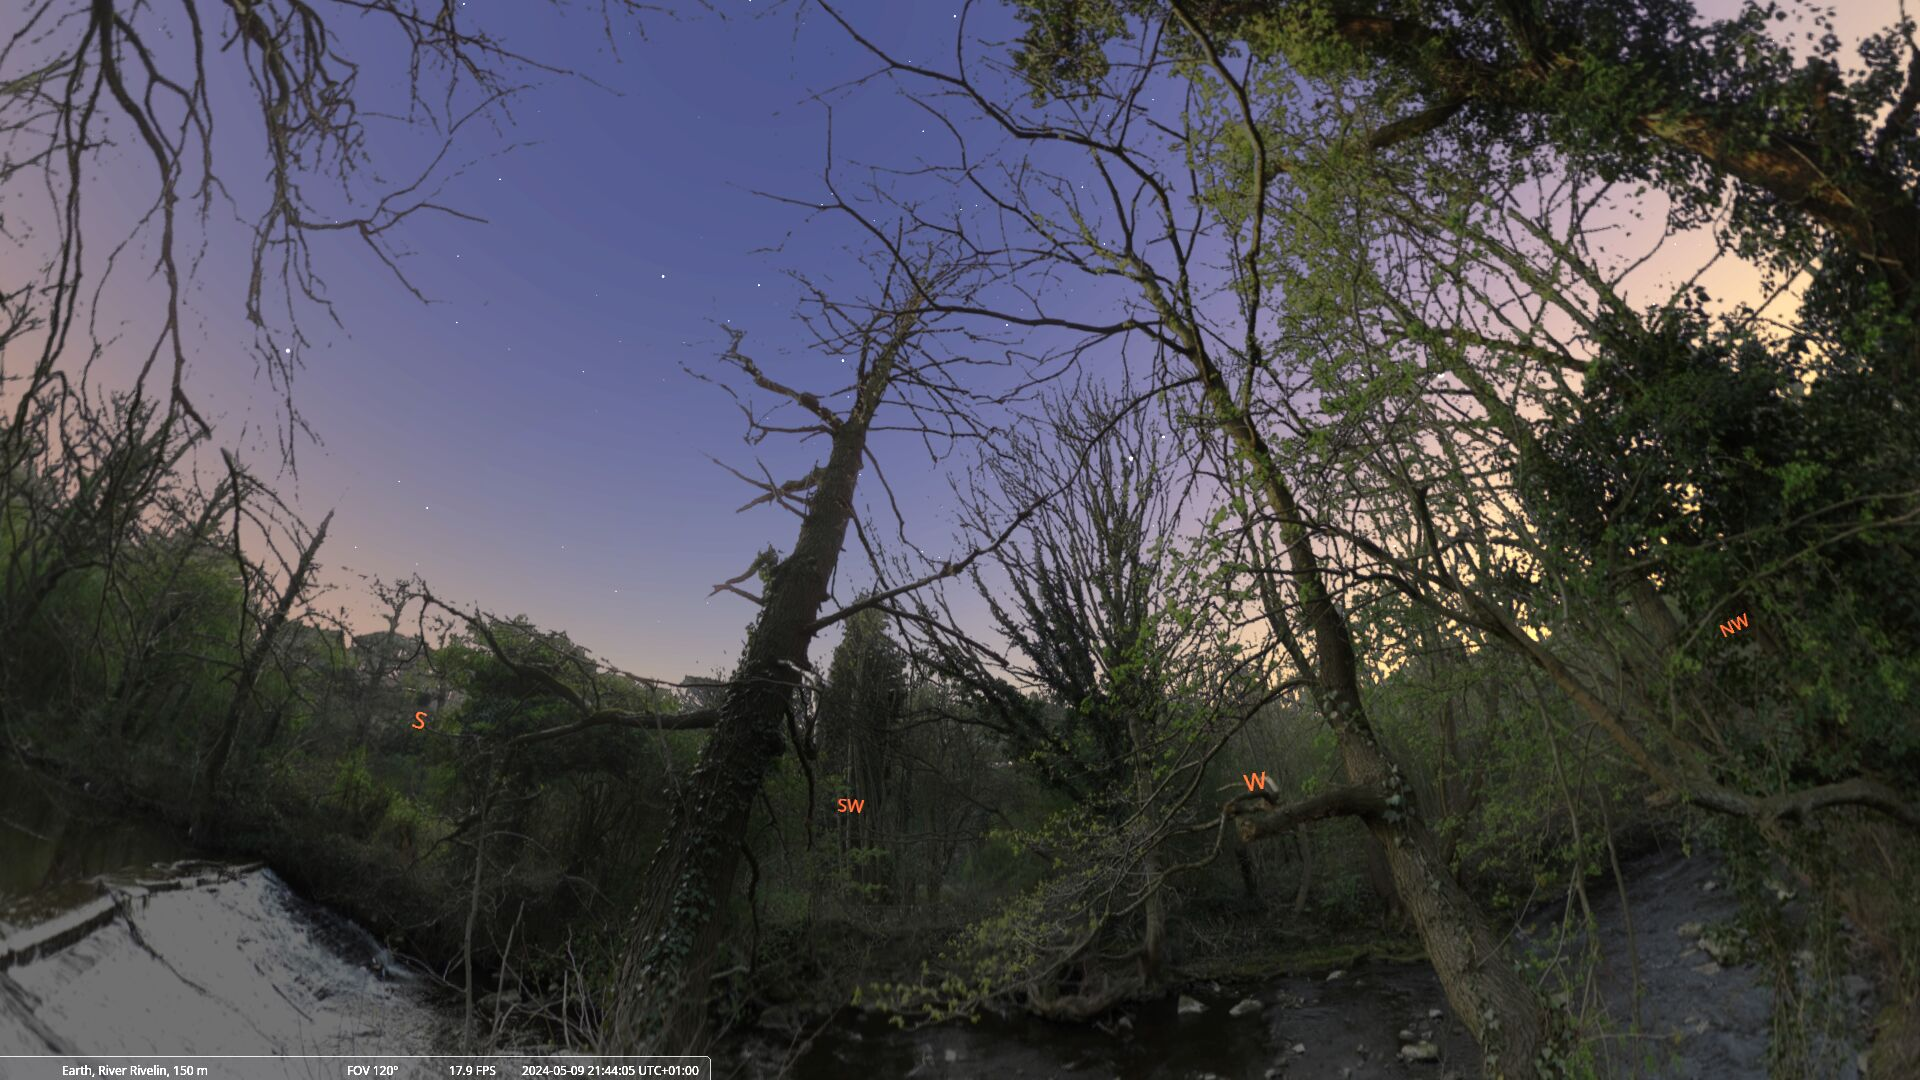
\includegraphics{stellarium}}\\
        Stellarium
      \end{center}
    \end{minipage}\bigskip\\
    \begin{minipage}[c]{.47\textwidth}
      \begin{center}
        \resizebox*{\textwidth}{!}{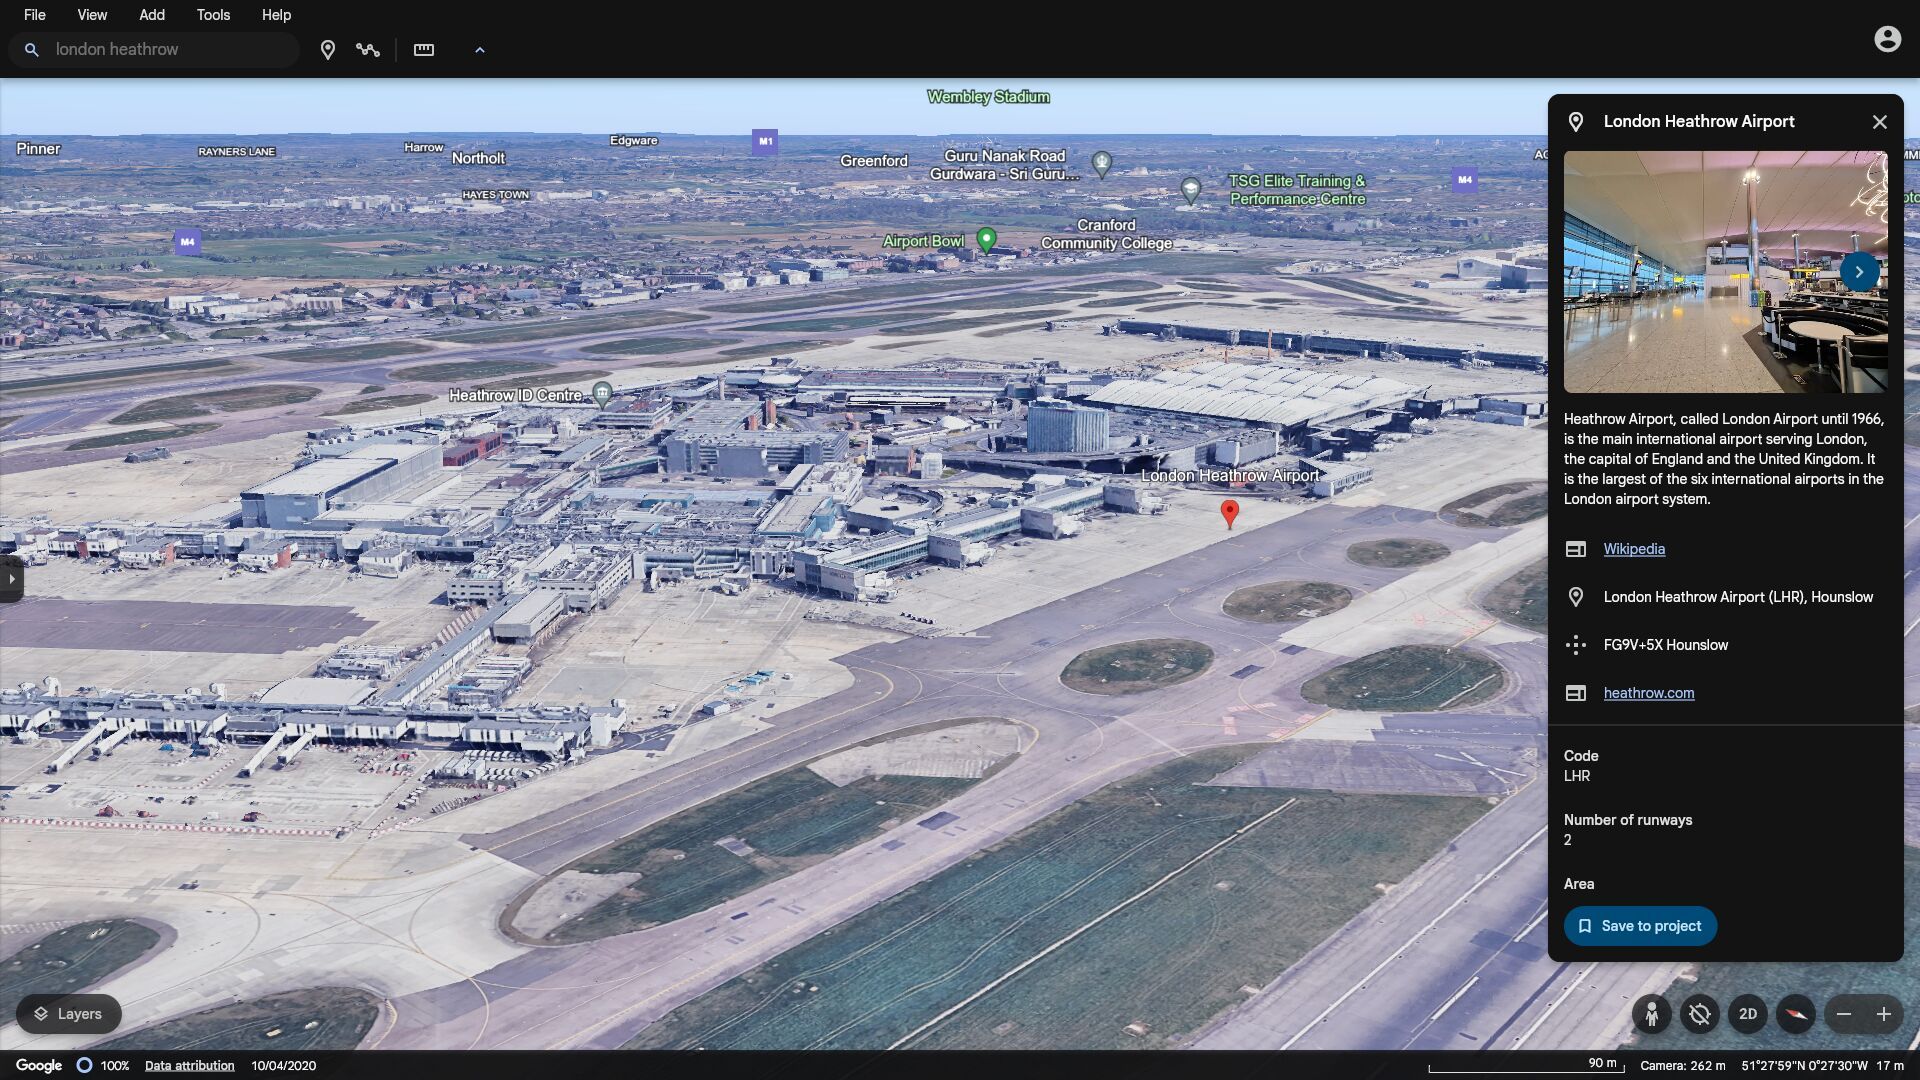
\includegraphics{google-earth}}\\
        WebGL (e.g. Google Earth)
      \end{center}
    \end{minipage}
    \begin{minipage}[c]{.47\textwidth}
      \begin{center}
        \resizebox*{\textwidth}{!}{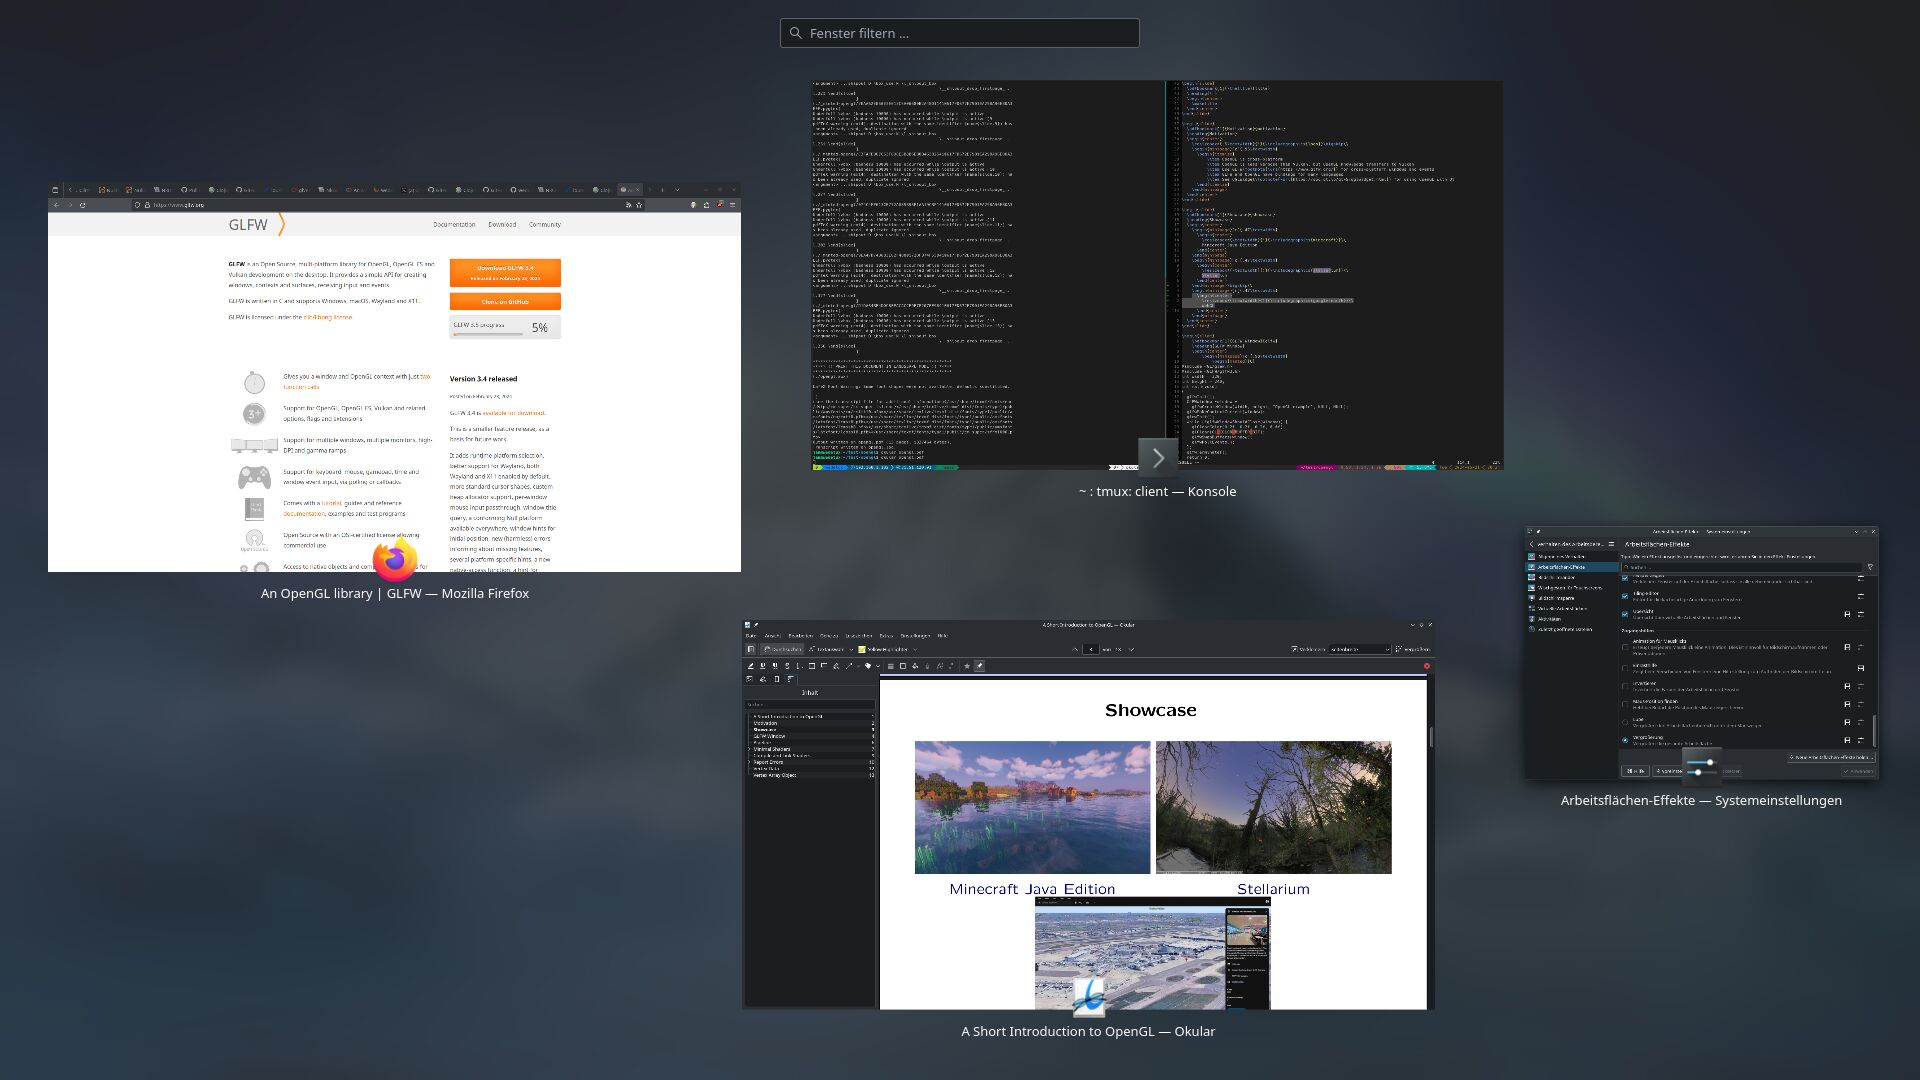
\includegraphics{kde}}\\
        KDE Plasma desktop
      \end{center}
    \end{minipage}
  \end{center}
\end{slide}

\begin{slide}
  \pdfbookmark[1]{GLFW}{glfw}
  \heading{GLFW}
  \begin{center}
    \resizebox*{\textwidth}{!}{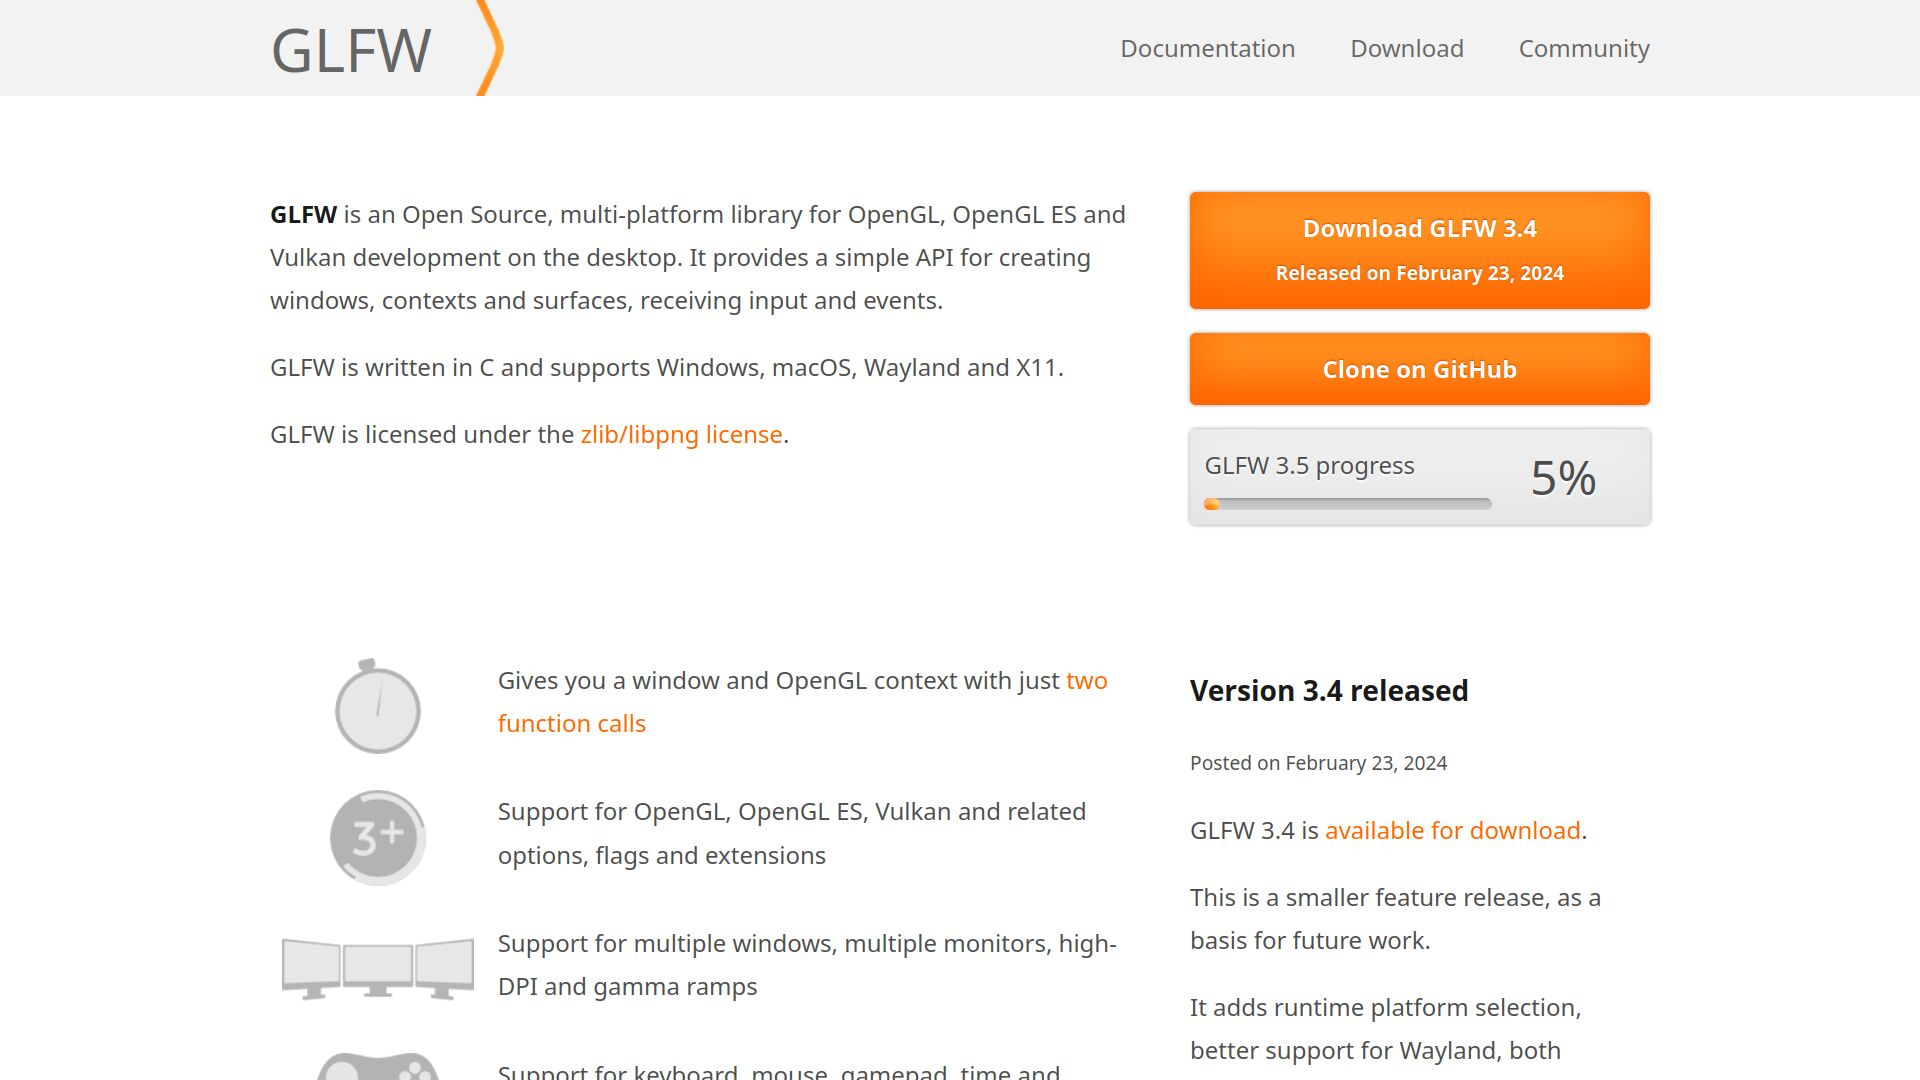
\includegraphics{glfw}}\\
  \end{center}
\end{slide}

\begin{slide}
    \pdfbookmark[1]{GLFW Window}{glfw}
    \heading{GLFW Window}
    \begin{center}
        \begin{minipage}[c]{.98\textwidth}
            \begin{minted}{C}
#include <GL/glew.h>
#include <GLFW/glfw3.h>
int width = 320;
int height = 240;
int main(void)
{
  glfwInit();
  GLFWwindow *window =
    glfwCreateWindow(width, height, "OpenGL example", NULL, NULL);
  glfwMakeContextCurrent(window);
  glewInit();
  while (!glfwWindowShouldClose(window)) {
    glClearColor(0.2f, 0.2f, 0.2f, 0.0f);
    glClear(GL_COLOR_BUFFER_BIT);
    glfwSwapBuffers(window);
    glfwPollEvents();
  };
  glfwTerminate();
  return 0;
}
            \end{minted}
        \end{minipage}
    \end{center}
\end{slide}

\begin{slide}
    \heading{GLFW Window}
    \begin{center}
      \resizebox*{.9\textwidth}{!}{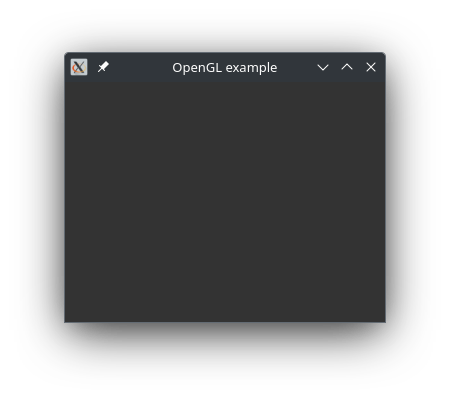
\includegraphics{glfw-window}}
    \end{center}
\end{slide}

\begin{slide}
  \pdfbookmark[1]{Pipeline}{pipeline}
  \heading{Pipeline}
  \begin{center}
    \begin{minipage}[t]{.45\textwidth}
        \subheading{minimal pipeline}\\
        \resizebox*{\textwidth}{!}{
\includegraphics{pipeline-minimal}}
    \end{minipage}
    \begin{minipage}[t]{.45\textwidth}
        \subheading{full pipeline}\\
        \resizebox*{\textwidth}{!}{
\includegraphics{pipeline}}
    \end{minipage}
  \end{center}
\end{slide}

\begin{slide}
    \pdfbookmark[1]{Minimal Shaders}{shader}
    \pdfbookmark[2]{Embedded in C}{shader}
    \heading{Minimal Shaders (Embedded in C)}
    \begin{center}
        \begin{minipage}[c]{.7\textwidth}
            \begin{minted}{C}
const char *vertexSource = "#version 130\n\
in mediump vec3 point;\n\
void main()\n\
{\n\
  gl_Position = vec4(point, 1);\n\
}";

const char *fragmentSource = "#version 130\n\
out mediump vec3 fragColor;\n\
void main()\n\
{\n\
  fragColor = vec3(1, 0, 0);\n\
}";
            \end{minted}
        \end{minipage}
    \end{center}
\end{slide}

\begin{slide}
    \pdfbookmark[2]{OpenGL Shader Language}{glsl}
    \heading{Minimal Shaders (OpenGL Shader Language (GLSL))}
    \begin{center}
        \begin{minipage}[c]{.5\textwidth}
            \begin{minted}{glsl}
#version 130
in mediump vec3 point;
void main()
{
  gl_Position = vec4(point, 1);
}
            \end{minted}
            \rule{4cm}{0.4pt}
            \begin{minted}{glsl}
#version 130
out mediump vec3 fragColor;
void main()
{
  fragColor = vec3(1, 0, 0);
}
            \end{minted}
        \end{minipage}
    \end{center}
\end{slide}

\begin{slide}
    \pdfbookmark[1]{Compile and Link Shaders}{compile}
    \heading{Compile \& Link Shaders}
    \begin{center}
        \begin{minipage}[c]{.95\textwidth}
            \begin{minted}{C}
// ...
int main(int argc, char** argv)
  // ...
  GLuint vertexShader = glCreateShader(GL_VERTEX_SHADER);
  glShaderSource(vertexShader, 1, &vertexSource, NULL);
  glCompileShader(vertexShader);
  handleCompileError("Vertex shader", vertexShader);

  GLuint fragmentShader = glCreateShader(GL_FRAGMENT_SHADER);
  glShaderSource(fragmentShader, 1, &fragmentSource, NULL);
  glCompileShader(fragmentShader);
  handleCompileError("Fragment shader", fragmentShader);

  GLuint program = glCreateProgram();
  glAttachShader(program, vertexShader);
  glAttachShader(program, fragmentShader);
  glLinkProgram(program);
  handleLinkError("Shader program", program);
  // ...
            \end{minted}
        \end{minipage}
    \end{center}
\end{slide}

\begin{slide}
    \pdfbookmark[1]{Report Errors}{report-errors}
    \pdfbookmark[2]{Compile Errors}{compile-error}
    \heading{Report Errors}
    \subheading{Compile Errors}
    \begin{center}
        \begin{minipage}[c]{.95\textwidth}
            \begin{minted}{C}
#include <stdio.h>
// ...
void handleCompileError(const char *step, GLuint context)
{
  GLint result = GL_FALSE;
  glGetShaderiv(context, GL_COMPILE_STATUS, &result);
  if (result == GL_FALSE) {
    char buffer[1024];
    glGetShaderInfoLog(context, 1024, NULL, buffer);
    if (buffer[0]) fprintf(stderr, "%s: %s\n", step, buffer);
  };
}
// ...
            \end{minted}
        \end{minipage}
    \end{center}
\end{slide}

\begin{slide}
    \pdfbookmark[2]{Link Errors}{link-error}
    \heading{Report Errors}
    \subheading{Link Errors}
    \begin{center}
        \begin{minipage}[c]{.95\textwidth}
            \begin{minted}{C}
#include <stdio.h>
// ...
void handleLinkError(const char *step, GLuint context)
{
  GLint result = GL_FALSE;
  glGetProgramiv(context, GL_LINK_STATUS, &result);
  if (result == GL_FALSE) {
    char buffer[1024];
    glGetProgramInfoLog(context, 1024, NULL, buffer);
    if (buffer[0]) fprintf(stderr, "%s: %s\n", step, buffer);
  };
}
// ...
            \end{minted}
        \end{minipage}
    \end{center}
\end{slide}

\begin{slide}
    \pdfbookmark[1]{Vertex Data}{vertex-data}
    \heading{Vertex and Index Data}
    \begin{center}
        \begin{minipage}[b]{.55\textwidth}
            \begin{minted}{C}
// ...
GLfloat vertices[] = {
  -0.5f, -0.5f,  0.0f,
   0.5f, -0.5f,  0.0f,
  -0.5f,  0.5f,  0.0f,
   0.5f,  0.5f,  0.0f
};

unsigned int indices[] = {0, 1, 3, 2};

GLuint vao;
GLuint vbo;
GLuint idx;
// ...
            \end{minted}
        \end{minipage}
        \begin{minipage}[b]{.4\textwidth}
          \resizebox*{.9\textwidth}{!}{
\includegraphics{ndc}}\\
          normalised device coordinates (NDC)
        \end{minipage}
    \end{center}
\end{slide}

\begin{slide}
    \pdfbookmark[1]{Vertex Array Object}{vao-data}
    \heading{Vertex Array Object}
    \begin{center}
        \begin{minipage}[c]{.95\textwidth}
            \begin{minted}{C}
  glGenVertexArrays(1, &vao);
  glBindVertexArray(vao);

  glGenBuffers(1, &vbo);
  glBindBuffer(GL_ARRAY_BUFFER, vbo);
  glBufferData(GL_ARRAY_BUFFER, sizeof(vertices), vertices,
               GL_STATIC_DRAW);
  glGenBuffers(1, &idx);
  glBindBuffer(GL_ELEMENT_ARRAY_BUFFER, idx);
  glBufferData(GL_ELEMENT_ARRAY_BUFFER, sizeof(indices), indices,
               GL_STATIC_DRAW);

  glVertexAttribPointer(glGetAttribLocation(program, "point"),
                        3, GL_FLOAT, GL_FALSE,
                        3 * sizeof(float), (void *)0);

  glUseProgram(program);
  glEnableVertexAttribArray(0);
            \end{minted}
        \end{minipage}
    \end{center}
\end{slide}

\begin{slide}
    \pdfbookmark[1]{Render Quads}{render-quads}
    \heading{Render Quads}
    \begin{center}
        \begin{minipage}[c]{.95\textwidth}
            \begin{minted}{C}
  // ...
  while (!glfwWindowShouldClose(window)) {
    glfwGetWindowSize(window, &width, &height);
    glViewport(0, 0, width, height);
    glClearColor(0.2f, 0.2f, 0.2f, 0.0f);
    glClear(GL_COLOR_BUFFER_BIT);
    glUseProgram(program);
    glBindVertexArray(vao);
    glDrawElements(GL_QUADS, 4, GL_UNSIGNED_INT, (void *)0);
    glfwSwapBuffers(window);
    glfwPollEvents();
  };
  // ...
            \end{minted}
        \end{minipage}
    \end{center}
\end{slide}

\begin{slide}
    \heading{Render Quads}
    \begin{center}
      \resizebox*{.9\textwidth}{!}{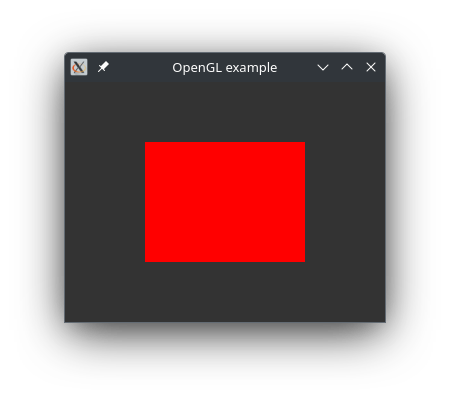
\includegraphics{quad}}
    \end{center}
\end{slide}

\begin{slide}
    \pdfbookmark[1]{Clean Up}{clean-up}
    \heading{Clean Up}
    \begin{center}
        \begin{minipage}[c]{.7\textwidth}
            \begin{minted}{C}
  // ...
  glDisableVertexAttribArray(0);

  glBindBuffer(GL_ELEMENT_ARRAY_BUFFER, 0);
  glDeleteBuffers(1, &idx);

  glBindBuffer(GL_ARRAY_BUFFER, 0);
  glDeleteBuffers(1, &vbo);

  glBindVertexArray(0);
  glDeleteVertexArrays(1, &vao);

  glDeleteProgram(program);
  glDeleteShader(vertexShader);
  glDeleteShader(fragmentShader);

  glfwTerminate();
  // ...
            \end{minted}
        \end{minipage}
    \end{center}
\end{slide}

% Depth buffer, enable depth-testing Reversed-z rendering
% homogeneous coordinates
% Projection matrix
% uniform matrix variable for rotation
% create cube with normals
% Phong shading
% Map dice texture (load image with STB?)
% Culling
% Tessellation
% Shadow mapping
% fog
% OpenGL superbible
% learnopengl.com

\end{document}
